% Made up for the tikra benchmark.
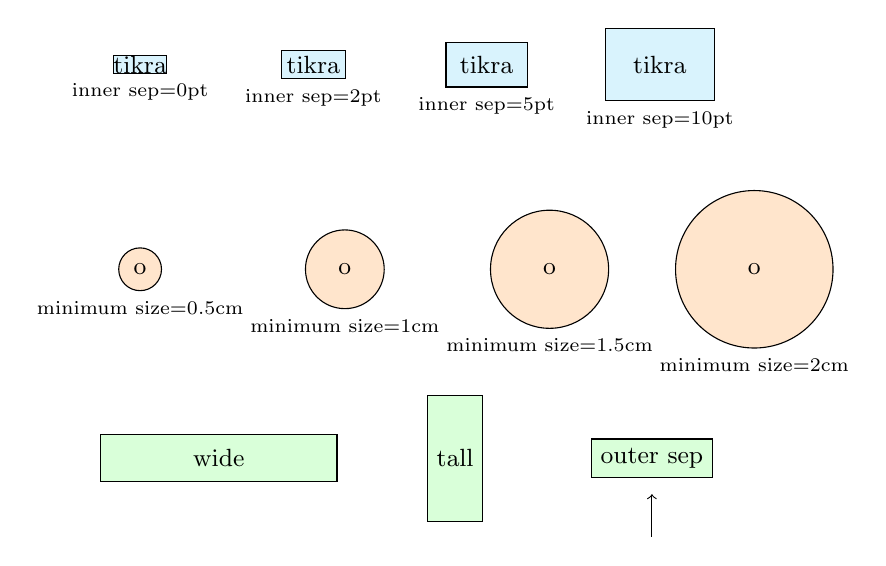
\begin{tikzpicture}[font=\small]
  \foreach \s [count=\i from 0] in {0pt, 2pt, 5pt, 10pt}
    \node[draw, fill=cyan!15, inner sep=\s, label=below:{\scriptsize inner sep=\s}] at (\i*2.2,0) {tikra};
  \foreach \m [count=\i from 0] in {0.5, 1, 1.5, 2}
    \node[draw, circle, fill=orange!20, minimum size=\m cm, label=below:{\scriptsize minimum size=\m cm}] at (\i*2.6,-2.6) {o};
  \node[draw, fill=green!15, minimum width=3cm, minimum height=0.6cm] at (1,-5) {wide};
  \node[draw, fill=green!15, minimum width=0.6cm, minimum height=1.6cm] at (4,-5) {tall};
  \node[draw, fill=green!15, outer sep=6pt] (o) at (6.5,-5) {outer sep};
  \draw[->] (6.5,-6) -- (o);
\end{tikzpicture}
